%---------------------------------------------------------def trazal---------------------------------------------------------------
    
%\begin{definition}   \textbf{Hiperplano.}   Un \emph{hiperplano} en \(\mathbb{R}^n\) es un subconjunto afín de dimensión \(n-1\). Más concretamente, dados un %vector no nulo \(\mathbf{a}\in\mathbb{R}^n\) y un escalar \(b\in\mathbb{R}\), el hiperplano asociado se define como
%\[
%H = \{\,\mathbf x\in\mathbb{R}^n : \langle \mathbf{a},\mathbf{x}\rangle = b\},
%\]
%donde \(\langle \mathbf{a},\mathbf{x}\rangle = a_1 x_1 + a_2 x_2 + \cdots + a_n x_n\) es el producto escalar en \(\mathbb{R}^n\).  En \(\mathbb{R}^3\) los %hiperplanos son los planos, ver definici\'on (\ref{plano}).
%\end{definition} 
    

%\begin{definition}\textbf{Traza.} 
%Se llama \emph{traza} de un conjunto \( S \subseteq \mathbb{R}^n \) a la intersección de \( S \) con un hiperplano \( H \subseteq \mathbb{R}^n \). 
%\end{definition}


%A continuaci\'on, definiremos unas Trazas particulares llamadas  \textbf{Conjunto de nivel}  y  \textbf{Cortes transversales} para conjuntos dados por g\'raficas de %funciones ( \ref{def:grafica})  


%---------------------------------------------------------def conjunto de nivel----------------------------------------------------
\begin{definition} \textbf{Conjunto de nivel.} 
    \label{def:conjunto de nivel}     
    Sea $f: U  \subseteq  \mathbb{R}^n \rightarrow \mathbb{R}$ y sea $c \in \mathbb{R}$, se define  \emph{el conjunto de nivel de $f$ de nivel}  $c$, y se nota $C(c,f)$,  como  
    \[
    C(c,f)=\{ \mathbf{x} \in U \;|\; f (\mathbf{x})=c \}.
     \]
 Es decir,  $C(c,f)$ es el conjunto de puntos $\vect{x}\in\ U$ para los cuales $f(x)=c$, o dicho de otra manera,  $C(c,f)$ es la preimagen de $c$ por $f$.   Llamaremos a los conjuntos de nivel por \emph{ curva de nivel}  o   \emph{superficie de nivel}, si $n=2$ o si $n=3$ respectivamente.   
\end{definition}


\begin{obs}  Si $f: U \subseteq \mathbb{R}^n \rightarrow \mathbb{R}$ entonces $C(c,f)   \subseteq  \mathbb{R}^{n}.$   Con el objetivo de poder dibujar,  nos detendremos en los casos $n=2$ y $n=3$  cuya definici\'on se desprende automaticamente  de la definici\'on  (\ref{def:conjunto de nivel}), es decir, 
 \begin{align}\label{def:conjunto de nive perticular} 
    C(c,f)&=\{ (x,y) \in U \;|\; f (x,y)=c \} \mbox{ si } n=2. \\
     C(c,f)&=\{ (x,y,z) \in U \;|\; f (x,y,z)=c \} \mbox{ si } n=3.
  \end{align} 
\end{obs}


\begin{definition} \textbf{Corte transversal.}   Sea $f: U  \subseteq  \mathbb{R}^2 \rightarrow \mathbb{R}$ y sea $a \in \mathbb{R}$, se define  \emph{el corte tranversal $f$}  con el plano vertical $x=a$, al conjunto
    \[
    \{   (x,y,z) \in \mathbb{R}^{3} \;|\; x=a \; ;\;   f (a,y)=z \},
     \] analogamente,  si $b \in \mathbb{R}$, se define  \emph{el corte tranversal $f$}  con el plano vertical $y=b$, al conjunto
    \[
    \{   (x,y,z) \in \mathbb{R}^{3} \;|\; y=b \; ;\;   f (x,b)=z \}.
     \]
\end{definition}


%----------------------------------------------------------ejemplos--------------------------------------------------------------

\begin{example}\label{example:ex1graf}   Sea  el campo  $f: \mathbb{R}^{2} \rightarrow \mathbb{R} \:|\:  f(x,y)=x^2+y^2.$ Hallar y graficar,  los conjuntos de nivel de $f$ y los cortes transversales  de  $\text{Graf}(f)$ con los planos de ecuaciones $x=0$ y $y=0$ . Hacer un dibujo de  $\text{Graf}(f)$.

        
Dado $c \in \mathbb{R}$, por (\ref{def:conjunto de nive perticular}), sabemos que 
     $$C(c,f)=\{(x,y) \in (\mathbb{R}^2 \;|\;   x^2+y^2  =c \}.$$

Tomemos, para ilustrar,  $c=0$, $c=1$ y $c=4$, 
    % quedando (ver (\ref{circ})) 
\begin{align*}   
C(0,f)&=\{(x,y) \in U \;|\; x^2+y^2=0 \}=\{(0,0) \} \\
C(1,f)&=\{(x,y) \in U \;|\; x^2+y^2=1 \} \\
C(4,f)&=\{(x,y) \in U \;|\; x^2+y^2=4 \}.
\end{align*}    
    

 \begin{figure}[H]  
\begin{center}
    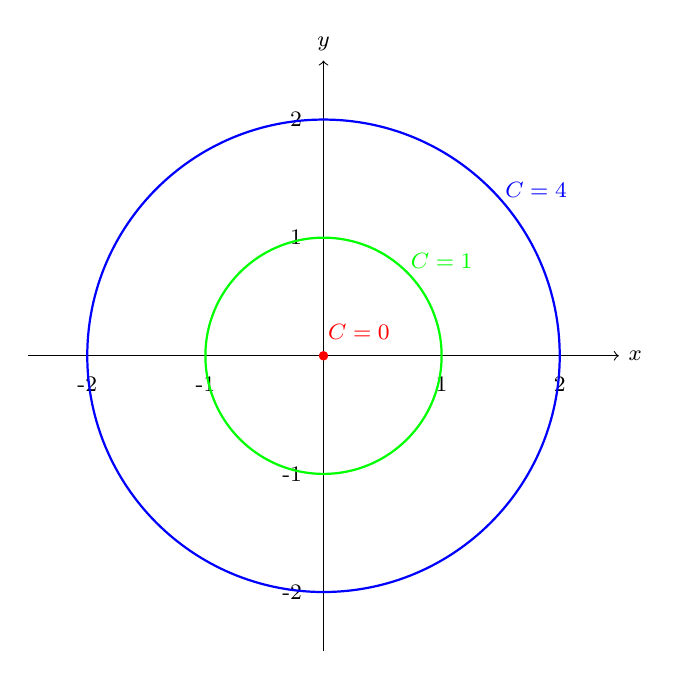
\begin{tikzpicture}[scale=1.5]
        % Dibujar ejes coordenados con números
        \draw[->] (-2.5,0) -- (2.5,0) node[right] {\footnotesize $x$};
        \draw[->] (0,-2.5) -- (0,2.5) node[above] {\footnotesize $y$};
        
        % Marcas y etiquetas en los ejes
        \foreach \x in {-2,-1,1,2}
            \draw (\x,0.1) -- (\x,-0.1) node[below] {\footnotesize \x};
        \foreach \y in {-2,-1,1,2}
            \draw (0.1,\y) -- (-0.1,\y) node[left] {\footnotesize \y};
        
        % Dibujar los círculos de nivel en sentido antihorario
        \draw[thick, green] (0,0) circle (1);
        \draw[thick, blue] (0,0) circle (2);

        
        % Etiquetas de los conjuntos de nivel
        \node[green] at (1,0.8) {\footnotesize $C=1$};
        \node[blue] at (1.8,1.4) {\footnotesize$C=4$};
        \node[red] at (0.3,0.2) {\footnotesize $C=0$};
        
        % Punto en el origen
        \filldraw[red] (0,0) circle (1pt);
    \end{tikzpicture}
\end{center}
  \caption{En rojo,  verde y azul  los conjuntos $C(0,f)$, $C(1,f)$ y $C(4,f)$, respectivamente.}
        %\label{fig:unitCircle1} 
   \end{figure}

    
    En general, podemos escribir a los conjuntos de nivel de $f$ como: 
       \[
            C(c,f)=
            \begin{dcases}
               x^2+y^2=c  &  c>0 \\
    (0,0)  & c=0\\
    \varnothing  & c<0.\\
            \end{dcases}
        \]

 Cada punto \( (x,y)\in  C(c,f)\)  se eleva al espacio como \((x,y,c)\),  colocándolo en el plano horizontal \(z = c\), generando un conjunto en el espacio.  El total de dichos conjuntos en distintos niveles \(c\) reconstruye una aproximación de la gráfica de $f$. En nuestro caso, podemos pensar a estos conjuntos como cortes entre la $\text{Graf}(f)$  y los planos horizontales $z=0$, $z=1$ y $z=4$ en $\mathbb{R}^{3}$, obteniendo

 \begin{figure}[H] 
\begin{center}
        %\begin{tabular}{cc}
            \begin{minipage}{0.45\textwidth}
              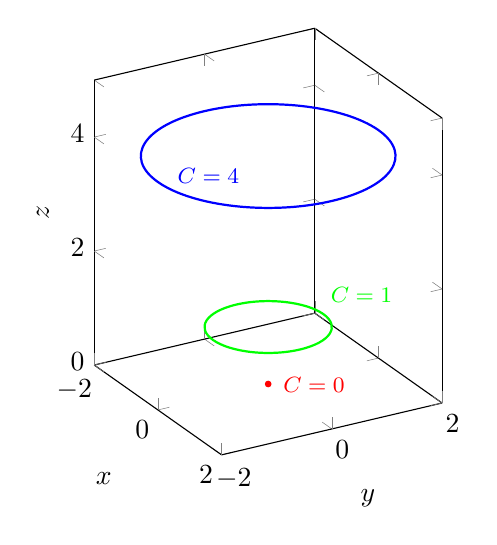
\begin{tikzpicture}
                  \begin{axis}[
                    view={60}{20},
                      xlabel={$x$},
                      ylabel={$y$},
                       zlabel={$z$},
                        xmin=-2, xmax=2,
                        ymin=-2, ymax=2,
                        zmin=0, zmax=5,
                       samples=50,
                       width=6cm,
                        height=7cm,
                        colormap/viridis
                    ]
                       \draw[thick, green] (0,0,1) circle (1);
                        \draw[thick, blue] (0,0,4) circle (2);
                        \node[green] at (1.2,1,1.8) {\footnotesize $C=1$};
                        \node[blue] at (0.2,-1.2,4) {\footnotesize $C=4$};
                        \node[red] at (0.4,0.6) {\footnotesize $C=0$};
                        \filldraw[red] (0,0) circle (1pt);
                    \end{axis}
                \end{tikzpicture}
            \end{minipage}
\end{center}
 \caption{En rojo,  verde y azul  los cortes de $\text{Graf}(f)$  con los planos horizontales $z=0$, $z=1$ y $z=4$, respectivamente.}
        %\label{fig:unitCircle1} 
  \end{figure}


Tomemos el corte transversal con el plano vertival $x=0$ y se deja al lector analizar el corte  $y=0.$  Para ello, observemos que, si $x=0$

$$z=f(0,y)=y^2.$$

\begin{figure}[H]
\begin{center}
    \begin{tikzpicture}
        % Ejes coordenados
        \draw[->] (-2.5,0) -- (2.5,0) node[right] {\footnotesize $y$};
        \draw[->] (0,-0.5) -- (0,4.5) node[above] {\footnotesize $z$};

        % Marcas en los ejes
        \foreach \x in {-2,-1,1,2}
            \draw (\x,0.1) -- (\x,-0.1) node[below] {\footnotesize \x};
        \foreach \y in {1,2,3,4}
            \draw (0.1,\y) -- (-0.1,\y) node[left] {\footnotesize \y};

        % Gráfica de f(y) = y^2
        \draw[domain=-2:2, smooth, variable=\y, blue, thick] 
            plot ({\y}, {\y*\y});

        % Etiqueta de la curva
        \node[blue] at (2, 1.6) {$z = y^2$};
    \end{tikzpicture}
\end{center}
 \caption{En  azul la relaci\'on $z=y^{2}$ y $x=0.$  }
        %\label{fig:unitCircle1} 
  \end{figure}

 Por \'ultimo, uniendo la informaci\'on hasta aca conseguida, tenemos que la gr\'afica de $f$ es

 \begin{figure}[H]
\begin{center}
    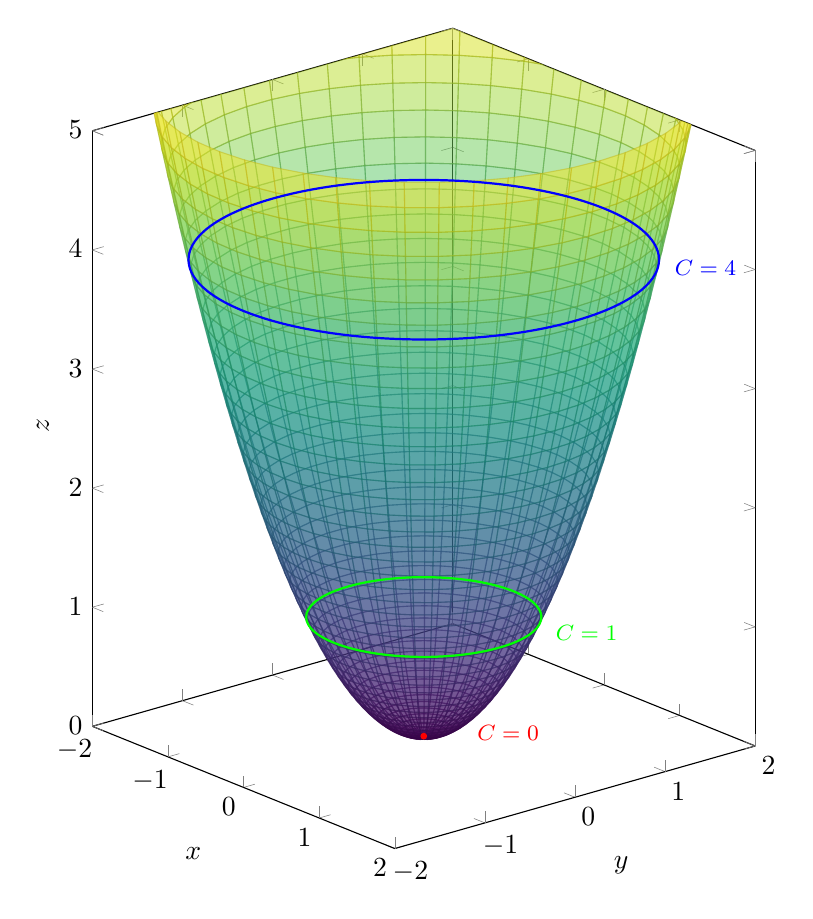
\begin{tikzpicture}
        \begin{axis}[
            view={50}{15},
            xlabel={$x$},
            ylabel={$y$},
            zlabel={$z$},
            xmin=-2, xmax=2,
            ymin=-2, ymax=2,
            zmin=0, zmax=5,  % Extender el eje z hasta 5
            samples=50,
            width=10cm,
            height=12cm,
            colormap/viridis
        ]
            \addplot3 [
                surf, opacity=0.5, draw=none, 
                restrict z to domain=0:5.6,
                data cs=polar, 
                domain=0:360, 
                y domain=0:{sqrt(5.9)}  % Ajustar el dominio radial
            ] 
            (x, y, y^2);
                % Dibujar los círculos de nivel en sentido antihorario
        \draw[thick, green] (0,0,1) circle (1);
        \draw[thick, blue] (0,0,4) circle (2);

     
        
        % Etiquetas de los conjuntos de nivel
        \node[green] at (1.2,0.8,1) {\footnotesize $C=1$};
        \node[blue] at (1.7,1.7,4) {\footnotesize $C=4$};
        \node[red] at (0.4,0.6) {\footnotesize $C=0$};
        
        % Punto en el origen
        \filldraw[red] (0,0) circle (1pt);
        \end{axis}
    \end{tikzpicture}
\end{center}
 \caption{Gr\'afica de la funci\'on $f$. }
        %\label{fig:unitCircle1} 
  \end{figure}
\end{example}


%\newpage     
    
\begin{example}\label{example:ej2graf} Para  el campo  $g: \mathbb{R}^{2} \rightarrow \mathbb{R} \;|\; g(x,y) = \sqrt{x^2+y^2},$  hallar y graficar,  los conjuntos de nivel de $g$ y los cortes transversales  de  $\text{Graf}(g)$ con los planos de ecuaciones $x=0$ y $y=0$ .  Hacer un dibujo de  $\text{Graf}(f)$.  




  
Dado $c \in \mathbb{R}$, por (\ref{def:conjunto de nive perticular}), sabemos que   $$C(c,g)=\{(x,y) \in U \;|\;   \sqrt{x^2+y^2}  =c \}.$$
    
Tomemos, para ilustrar,  $c=0$, $c=1$ y $c=2$, 
    % quedando (ver (\ref{circ})) 
    \[
        C(0,g)=\{(x,y) \in U \;|\; \sqrt{x^2+y^2}=0 \}
        \]
         \[
        C(1,g)=\{(x,y) \in U \;|\; \sqrt{x^2+y^2}=1 \}
        \]
         \[
        C(2,g)=\{(x,y) \in U \;|\; \sqrt{x^2+y^2}=2 \}.
         \]
    
    
  
    
\begin{figure}[H]
     \begin{center}
        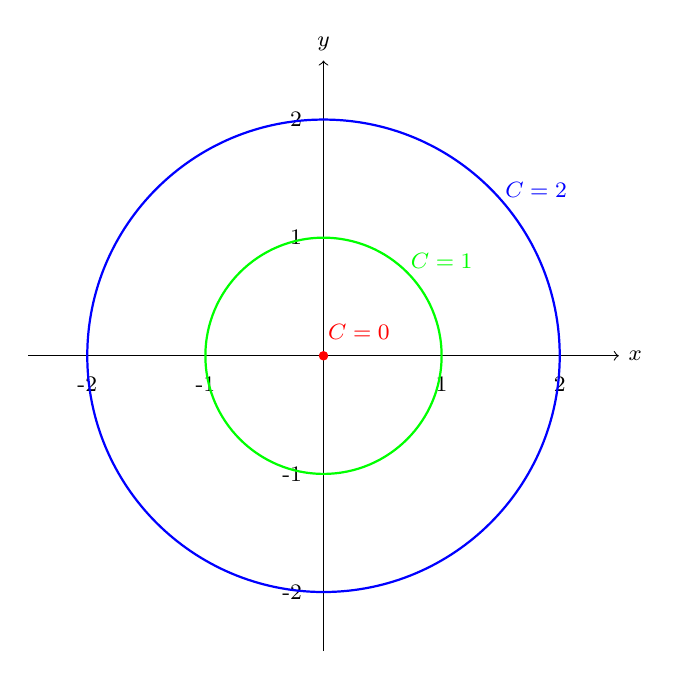
\begin{tikzpicture}[scale=1.5]
            % Dibujar ejes coordenados con números
            \draw[->] (-2.5,0) -- (2.5,0) node[right] {\footnotesize $x$};
            \draw[->] (0,-2.5) -- (0,2.5) node[above] {\footnotesize $y$};
            
            % Marcas y etiquetas en los ejes
            \foreach \x in {-2,-1,1,2}
                \draw (\x,0.1) -- (\x,-0.1) node[below] {\footnotesize \x};
            \foreach \y in {-2,-1,1,2}
                \draw (0.1,\y) -- (-0.1,\y) node[left] {\footnotesize \y};
            
            % Dibujar los círculos de nivel en sentido antihorario
            \draw[thick, green] (0,0) circle (1);
            \draw[thick, blue] (0,0) circle (2);
    
            
            % Etiquetas de los conjuntos de nivel
            \node[green] at (1,0.8) {\footnotesize $C=1$};
            \node[blue] at (1.8,1.4) {\footnotesize $C=2$};
            \node[red] at (0.3,0.2) {\footnotesize $C=0$};
            
            % Punto en el origen
            \filldraw[red] (0,0) circle (1pt);
        \end{tikzpicture}
  \end{center}
  \caption{En rojo,  verde y azul  los conjuntos $C(0,g)$, $C(1,g)$ y $C(4,g)$, respectivamente.}
        %\label{fig:unitCircle1} 
   \end{figure}
    
   En general, podemos escribir a los conjuntos de nivel de $g$ como:
       \[
            C(c,f)=
            \begin{dcases}
            \sqrt{ x^2+y^2}=c  &  c>0 \\
    (0,0)  & c=0\\
    \varnothing  & c<0.\\
            \end{dcases}
        \]
   

Analogamente al ejemplo anterior, podemos "elevar"  los  conjuntos $ C(c,f)$  a "altura"  $z=c$ y dibujarlos en  $\mathbb{R}^{3}$
 \begin{figure}[H]
\begin{center}
 \tikzsetnextfilename{Conjuntos-de-nivel-cono}  
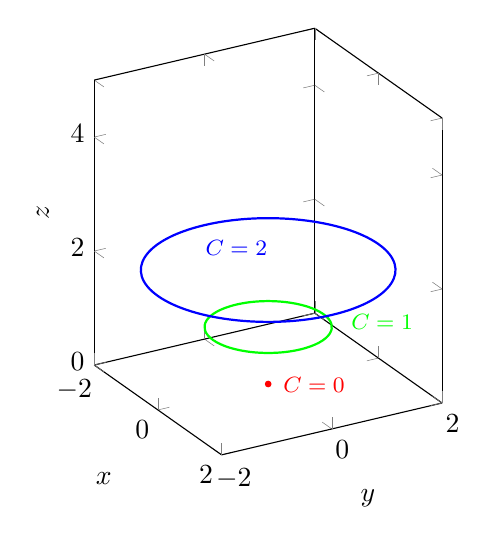
\begin{tikzpicture} 
                        \begin{axis}[
                        view={60}{20},
                        xlabel={$x$},
                        ylabel={$y$},
                        zlabel={$z$},
                        xmin=-2, xmax=2,
                        ymin=-2, ymax=2,
                        zmin=0, zmax=5,
                        samples=50,
                        width=6cm,
                        height=7cm,
                        colormap/viridis
                    ]
                    \draw[thick, green] (0,0,1) circle (1);
                    \draw[thick, blue] (0,0,2) circle (2);
            
                 
                    
                    % Etiquetas de los conjuntos de nivel
                    \node[green] at (1.5,1.2,1.4) {\footnotesize $C=1$};
                    \node[blue] at (-1,0,2) {\footnotesize $C=2$};
                    \node[red] at (0.4,0.6) {\footnotesize $C=0$};
                    
                    % Punto en el origen
                    \filldraw[red] (0,0) circle (1pt);
                    \end{axis}
                \end{tikzpicture}
        \end{center}
\caption{En rojo,  verde y azul  los cortes de la $\text{Graf}(f)$  con los planos horizontales $z=0$, $z=1$ y $z=2$, respectivamente.}
        %\label{fig:unitCircle1} 
  \end{figure}

%%%%%%%%%%%%%%%%%%%%%%%%%%%%%%%%%%%%%%%%%%%%%%%%%
Tomemos el corte transversal con el plano vertival $x=0$ y se deja al lector analizar el corte  $y=0.$  Para ello, observemos que, si $x=0$
$$z= f(0,y)=|y|$$

 \begin{figure}[H]
\begin{center}
    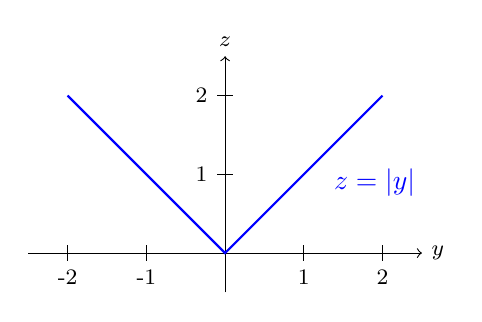
\begin{tikzpicture}
        % Ejes coordenados
        \draw[->] (-2.5,0) -- (2.5,0) node[right] {\footnotesize $y$};
        \draw[->] (0,-0.5) -- (0,2.5) node[above] {\footnotesize $z$};

        % Marcas en los ejes
        \foreach \x in {-2,-1,1,2}
            \draw (\x,0.1) -- (\x,-0.1) node[below] {\footnotesize \x};
        \foreach \y in {1,2}
            \draw (0.1,\y) -- (-0.1,\y) node[left] {\footnotesize \y};

        % Gráfica de f(y) = |y|
        \draw[thick, blue] (-2,2) -- (0,0) -- (2,2);

        % Etiqueta de la curva
        \node[blue, below, xshift=0.6cm] at (1.3, 1.2) {$z = |y|$};
    \end{tikzpicture}
\end{center}
 \caption{En   azul la relaci\'on $z=|y| $ y $x=0.$  }
        %\label{fig:unitCircle1} 
  \end{figure}


 Por \'ultimo, uniendo la informaci\'on hasta aca conseguida, tenemos que la gr\'afica de $g$ es
   
 \begin{figure}[H]
       \begin{center}
         %\tikzsetnextfilename 
          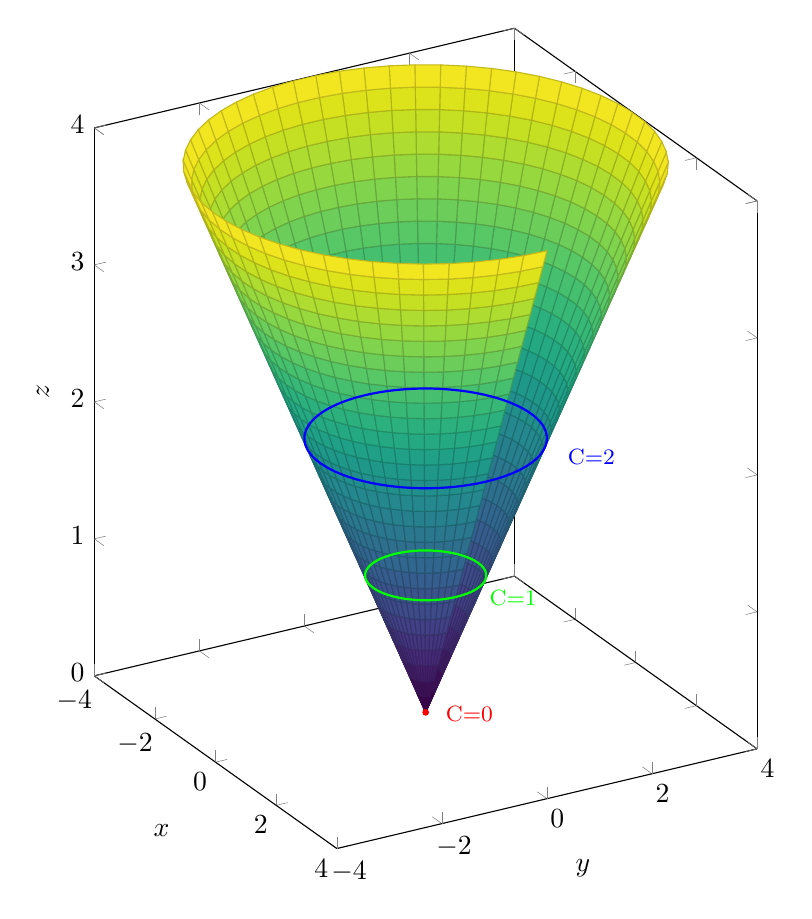
\begin{tikzpicture} 
                \begin{axis}[
                        view={60}{20},
                        xlabel=$x$,
                        ylabel=$y$,
                        zlabel=$z$,
                        xmin=-4,
                        ymin=-4,
                        zmin=0,
                        xmax=4,
                        ymax=4,
                        zmax=4,
                        samples=50,
                        width=10cm,
                        height=12cm,
                        colormap/viridis,
                    ]
                    \addplot3[
                surf,
                domain=0:4,
                y domain=0:360,
                samples=30,
                samples y=60
            ]
            ({x*cos(y)},{x*sin(y)},{x}); % Parámetrico: x = r cos(θ), y = r sin(θ), z = r
               % Dibujar los círculos de nivel en sentido antihorario
            \draw[thick, green] (0,0,1) circle (1);
            \draw[thick, blue] (0,0,2) circle (2);
    
         
            
            % Etiquetas de los conjuntos de nivel
            \node[green] at (1.5,0.8,1) {\footnotesize C=1};
            \node[blue] at (2,2,2) {\footnotesize C=2};
            \node[red] at (0.4,0.6) {\footnotesize C=0};
            
            % Punto en el origen
            \filldraw[red] (0,0) circle (1pt);
                \end{axis}
                
            \end{tikzpicture}
            
        \end{center}
   \caption{Gr\'afica de la funci\'on $g$.  }
        %\label{fig:unitCircle1} 
  \end{figure}
\end{example}
    
    
    \begin{obs} Dibujar todos los puntos en $\mathbb{R}^{3}$ tales que \( z^2 = x^2 + y^2 \).  si despejamos \( z \) obtenemos dos expresiones:
        \[
        z = \sqrt{x^2 + y^2} ,
        \quad
        z = -\sqrt{x^2 + y^2}.
        \]
        Definimos entonces las funciones:
        \[
        f_1 : \mathbb{R}^2 \to [0,+\infty), \quad f_1(x,y) = \sqrt{x^2 + y^2},
        \]
        \[
        f_2 : \mathbb{R}^2 \to (-\infty,0], \quad f_2(x,y) = -\sqrt{x^2 + y^2}.
        \]
        
        Así, los conjuntos de nivel de \( f_1 \) y \( f_2 \) son:
        \[
        C(c,f_1)=
        \begin{dcases}
        x^2+y^2=c  &  c>0 \\
        (0,0)  & c=0\\
        \varnothing  & c<0\\
        \end{dcases}
        \]
        \[
        C(c,f_2)=
        \begin{dcases}
        x^2+y^2=c  &  c<0 \\
        (0,0)  & c=0\\
        \varnothing  & c>0\\
        \end{dcases}
        \]

        De esta manera, considerando la definición de gráfica de una función, podemos representar en \(\mathbb{R}^3\) las gráficas de \( f_1 \) y \( f_2 \), que juntas forman el cono dado por la ecuación \( z^2 = x^2 + y^2 \).
        
        \begin{center}
            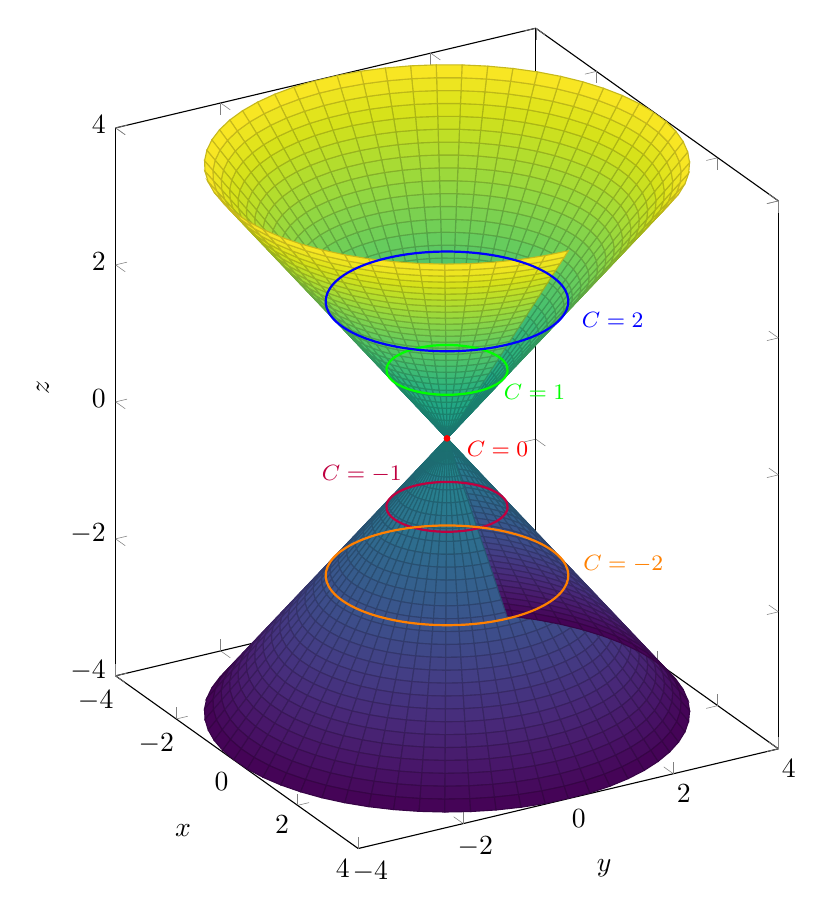
\begin{tikzpicture}
                \begin{axis}[
                        view={60}{20},
                        xlabel=$x$,
                        ylabel=$y$,
                        zlabel=$z$,
                        xmin=-4,
                        ymin=-4,
                        zmin=-4,
                        xmax=4,
                        ymax=4,
                        zmax=4,
                        samples=50,
                        width=10cm,
                        height=12cm,
                        colormap/viridis,
                    ]
                    % Cono superior
                    \addplot3[
                        surf,
                        domain=0:4,
                        y domain=0:360,
                        samples=30,
                        samples y=60
                    ]
                    ({x*cos(y)},{x*sin(y)},{x});
                    
                    % Cono inferior
                    \addplot3[
                        surf,
                        domain=0:4,
                        y domain=0:360,
                        samples=30,
                        samples y=60
                    ]
                    ({x*cos(y)},{x*sin(y)},{-x});
        
                    % Dibujar los círculos de nivel en sentido antihorario
                    \draw[thick, green] (0,0,1) circle (1);
                    \draw[thick, blue] (0,0,2) circle (2);
                    \draw[thick, purple] (0,0,-1) circle (1);
                    \draw[thick, orange] (0,0,-2) circle (2);
        
                    % Etiquetas de los conjuntos de nivel
                    \node[green] at (1.5,0.8,1) {\footnotesize $C=1$};
                    \node[blue] at (2,2,2) {\footnotesize $C=2$};
                    \node[purple] at (1,-2.2,0.2) {\footnotesize $C=-1$};
                    \node[orange] at (2,2.2,-1.6) {\footnotesize $C=-2$};
                    \node[red] at (0.8,0.5,0) {\footnotesize $C=0$};
                    
                    % Punto en el origen
                    \filldraw[red] (0,0,0) circle (1pt);
                \end{axis}
            \end{tikzpicture}
        \end{center}
        \end{obs}


  

 






